\chapter{Определение области применения и главных требований к разрабатываемым конвертерам}
\label{cha:analysis}
%
% % В начале раздела  можно напомнить его цель
%
В данном разделе поясняется область применения разрабатываемого ПО, а также, указываются требования к разрабатываемым конвертерам.

\section{Область применения ПО <<Primiview>>}

Конвертер в TXT по типу DXF применяется для контроля содержания необходимых (поддерживаемых) примитивов (объектов) в DXF-файле. Также, с помощью данного формата может производится расчёт длины траектории  контура детали (обычно, в поперечном её сечении). Это может быть полезно при применении ПО в области лазерной резки с помощью станков с ЧПУ, а, в частности, в ПО <<Сириус>>.

Конвертер из DXF в TXT в формате координат и радиуса применяется для автоматизированного технологического проектирования, для формирования УП. Получаемая в результате работы ПО информация о примитивах изображения контура детали используется для непосредственного составления УП, так как каждая последующая точка имеет не только плоские координаты, но и способ достижения этой точки (тип примитива: отрезок, если радиус равен нулю; дуга, если радиус ненулевой).

Конвертер в SVG-формат полезен для последующего формирования других типов файлов (например, DBS), а также, для компактного по объёму файла векторного представления контура детали. ИВЗУАЛИЗАЦИЯ. ПОДробно о svg - литературный обзор. Внутренняя репрезентация (ezdxf)

Конвертер в JSON удобен для хранения информации об объектах контура детали. В этом формате работает и другое ПО разрабатываемой САПР для формирования УП для станков с ЧПУ.

В целом, разрабатываемый набор конвертеров (модуль экспорта) представляет собой цельный ПП, сочетающий в себе набор необходимых разработчику УП начальных функций для автоматизированного технологического проектирования. Это ПО может быть интегрировано в разные ПП, так как по сути универсально в своём применении (используется в области 2D-резки, токарной обработке).



\section{Главные требования ко входному файлу}

Так как данная работа нацелена на создание ПО для обработки геометрической информации 2D-объектов специального типа, то конвертироваться из DXF-файлов должна не вся информация, содержащаяся в них. В первую очередь, заказчиком работы было определено, что на входе будет подаваться 2D-контур деталей типа <<Втулка>>, то есть тел вращения. Так как сконвертированная геометрия данных объектов в последующем предполагает разработку УП для токарных станков с ЧПУ, то геометрическая информация должна содержать определённый набор геометрических примитивов, с которым может работать система исполнительных органов станков с ЧПУ. Этот набор ограничивается тем, что исполнительные органы станков с ЧПУ способны перемещаться либо с помощью \textbf{линейной}, либо с помощью \textbf{круговой интерполяции}. Из этого следует, что для корректной работы САПР, для которых предназначаются разрабатываемые конвертеры, геометрия в DXF-файле на входе конвертеров должна состоять из, как минимум одного из представленных далее примитивов:

\begin{enumerate}
	\item линия (отрезок),
	\item полилиния,
	\item дуга,
	\item окружность.
\end{enumerate}

Остальные типы геометрии, реализуемой в формате DXF, такие как \textit{эллипс}, \textit{сплайн}, будут игнорироваться ПО.

\section{Описание формата DXF-файлов}\label{sec:allaboutdxf}

На вход разрабатываемому конвертеру подаётся файл формата DXF. Формат DXF представляет собой совокупность данных с тегами всей информации, содержащейся в файле чертежа AutoCAD. Тегированные данные означают, что каждому элементу данных в файле предшествует целое число, называемое групповым кодом. Значение группового кода указывает, какой тип данных имеет следующий элемент. Это значение также указывает смысл элемента данных для данного типа объекта. Практически вся указанная пользователем информация в файле чертежа может быть представлена в формате DXF \cite{Autodesk}.
В DXF файлах, в зависимости от их содержания, существуют сущности, представляющие для нас интерес. Среди них следующие:

\begin{enumerate}
	\item LINE (Линия),
	\item LWPOLYLINE (Полилиния),
	\item ARC (Дуга),
	\item CIRCLE (Окружность),
	\item INSERT (Вставка).
\end{enumerate}

Как уже и было отмечено, существуют и другие примитивы (ELLIPSE, SPLINE и др.), однако, основываясь на конкретных целях заказчика по возможности применения выходных файлов для генерации УП, ПП проектируется только с указанными примитивами и сущностями DXF.

Рассмотрим каждую из сущностей подробнее.

\paragraph{LINE.} Рассмотрим тэги сущности \textit{Линия}, необходимые для её реального отображения (см. табл. \ref{tab:line}).


\begin{longtable}{|l|l|}
	\caption{Рассматриваемые групповые коды сущности LINE}
	\label{tab:line}
	\centering
	\tabularnewline
	\hline
	Групповой код & Описание\\
	\hline \endfirsthead
	\subcaption{Продолжение таблицы~\ref{tab:line}}
	\\ \endhead
	\subcaption{Продолжение на след. стр.}
	\endfoot
	%\hline
	\endlastfoot
	39	&	Толщина (необязательный; по умолч. = 0)\\ \hline
	10	&	Начальная точка (в с.к. объекта) DXF: значение X\\ \hline
	20, 30	&	DXF: Y и Z значения начальной точки (в с.к. объекта)\\ \hline
	11	&	Конечная точка (в с.к. объекта)	DXF: значение X\\ \hline
	21, 31	&	DXF: Y и Z значения конечной точки (в с.к. объекта)\\ \hline
\end{longtable}

\paragraph{LWPOLYLINE.} Рассмотрим тэги сущности \textit{Полилиния}, необходимые для её реального отображения (см. табл. \ref{tab:polyline}).

\begin{longtable}{|p{70pt}|p{370pt}|}
	\caption{Рассматриваемые групповые коды сущности POLYLINE}
	\label{tab:polyline}
	\centering
	\tabularnewline
	\hline
	Групповой код & Описание\\
	\hline \endfirsthead
	\subcaption{Продолжение таблицы~\ref{tab:polyline}}
	\\ \endhead
	\subcaption{Продолжение на след. стр.}
	\endfoot
	%\hline
	\endlastfoot
	70	&	«Флаг» полилинии (бит-закодировано); по умолч. = 0; 1 – закрыта\\ \hline
	39	&	Толщина (необязательный; по умолч. = 0)\\ \hline
	10	&	Координаты вершин (в с.к. объекта), множественные вхождения; по одному вхождению для каждой вершины DXF: значение X\\ \hline
	20	&	DXF: значение Y координат вершин (в с.к. объекта), множественные вхождения; по одному вхождению для каждой вершины\\ \hline
	42	&	\textit{Bulge}. Выпуклость (множественные вхождения - для каждой вершины), (необязательно; по умолч. =0)\\ \hline	
\end{longtable}

\paragraph{ARC.} Рассмотрим тэги сущности \textit{Дуга}, необходимые для её реального отображения (см. табл. \ref{tab:arc}).

\begin{longtable}{|p{70pt}|p{370pt}|}
	\caption{Рассматриваемые групповые коды сущности ARC}
	\label{tab:arc}
	\centering
	\tabularnewline
	\hline
	Групповой код & Описание\\
	\hline \endfirsthead
	\subcaption{Продолжение таблицы~\ref{tab:arc}}
	\\ \endhead
	\subcaption{Продолжение на след. стр.}
	\endfoot
	%\hline
	\endlastfoot
	39	&	Толщина (необязательный; по умолч. = 0)\\ \hline	
	10	&	Центр дуги (в с.к. объекта)
	DXF: значение X\\ \hline	
	20, 30	&	DXF: Y и Z значения центра дуги (в с.к. объекта)\\ \hline	
	40	&	Радиус\\ \hline	
	50	&	Начальный угол\\ \hline	
	51	&	Конечный угол\\ \hline	
\end{longtable}

\paragraph{CIRCLE.} Рассмотрим тэги сущности \textit{Окружность}, необходимые для её реального отображения (см. табл. \ref{tab:circle}).

\begin{longtable}{|p{70pt}|p{370pt}|}
	\caption{Рассматриваемые групповые коды сущности CIRCLE}
	\label{tab:circle}
	\centering
	\tabularnewline
	\hline
	Групповой код & Описание\\
	\hline \endfirsthead
	\subcaption{Продолжение таблицы~\ref{tab:circle}}
	\\ \endhead
	\subcaption{Продолжение на след. стр.}
	\endfoot
	%\hline
	\endlastfoot
	39	&	Толщина (необязательный; по умолч. = 0)\\ \hline	
	10	&	Центр дуги (в с.к. объекта)
	DXF: значение X\\ \hline	
	20, 30	&	DXF: Y и Z значения центра дуги (в с.к. объекта)\\ \hline	
	40	&	Радиус\\ \hline	
	50	&	Начальный угол\\ \hline	
	51	&	Конечный угол\\ \hline	
\end{longtable}

\paragraph{INSERT.} Данная сущность представляет собой вставку блоков с геометрией. Её необходимо рассматривать, так как геометрия может быть вложенной и, таким образом, не видна обзорщиком сущностей, так как вложена. У этой сущности поиск информации по тэгам в программе не потребуются.

\section{Параметр <<bulge>>}\label{sec:bulge}

Особый интерес представляет параметр \textit{bulge} (выпуклость) для каждой из вершин полилинии.
Чтобы понять сущность данного параметра, который представляет собой некоторую степень кривизны дуги окружности между двумя точками, необходимо сначала разобраться с геометрией дуг.

\begin{figure}[H]
	\centering
	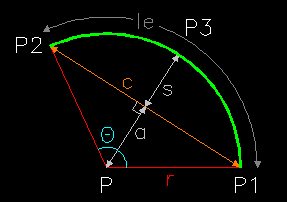
\includegraphics[width=0.5\textwidth]{figures/arcgeom.png}
	\captionof{figure}{Геометрия дуги окружности}
	\label{fig:arcgeom}
\end{figure}

Так как дуга окружности описывает часть этой окружности, то она и обладает всеми атрибутами данной окружности (см. рис. \ref{fig:arcgeom}). Среди них:

\begin{itemize}
	\item Радиус ($r$) --- радиус дуги такой же, как и у окружности;
	\item Центр ($P$) --- тот же, что и у окружности;
	\item Центральный угол ($\Theta$) --- в окружности равен $360^{\circ}$;
	\item Длина дуги ($le$) --- является частью периметра (длины) окружности.
\end{itemize}

Для дальнейшей работы с геометрией дуг примем, также, следующие специфичные атрибуты:

\begin{itemize}
	\item Начальная и конечная точка ($P1, P2$) --- это «вершины» дуги. Хотя иногда и целесообразно говорить о конкретных точках, не лежащих на концах дуги;
	\item Длина хорды ($c$) --- у дуг и окружностей можно провести бесконечное количество хорд, но для нас интерес представляет только хорда, проходящая через её вершины;
	\item Середина дуги ($P3$) --- точка, делящая дуги с данными вершинами на две, равные по длине, дуги;
	\item Апофема ($a$) --- это отрезок, вершинами которого являются середина дуги и её центр. Апофема перпендикулярна хорде;
	\item Высота дуги ($s$) --- это отрезок, проведённый из середины дуги перпендикулярно к хорде.
\end{itemize}

 Кроме самой себя, дуга может, также, и описывать другие геометрические формы: круговой сегмент и сектор. Обе геометрические формы включают в себя все вышеперечисленные атрибуты, однако для выведения формулы параметра \textit{bulge} (выпуклости), потребуется рассмотрение только кругового сектора.

В документации AutoCAD \cite{Autodesk} выпуклостью называется тангенс четверти угла дуги между выбранной вершиной и следующей вершиной в списках вершин полилиний. Отрицательность параметра \textit{bulge} указывает на то, что дуга отрисовывается по часовой стрелке от выбранной вершины к следующей. Выпуклость, равная нулю --- прямой сегмент, выпуклость, равная единице --- половина окружности.

Проблема «расшифровки» атрибутов дуги для дальнейших манипуляций с ней заключается в том, что входными данными являются только координаты вершин и рассматриваемый параметр --- \textit{bulge}.

В самом деле, взяв арктангенс от параметра \textit{bulge} и умножив его на $4$, легко получить центральный угол, на который опирается рассматриваемая дуга. Результат получен в радианах. Для перевода значения в градусы, необходимо умножить это значение на $\pi$ и разделить на $180^{\circ}$.

Для вывода данной зависимости, рассмотрим дугу окружности (см. рис. \ref{fig:arcchord}).

\begin{figure}[H]
	\centering
	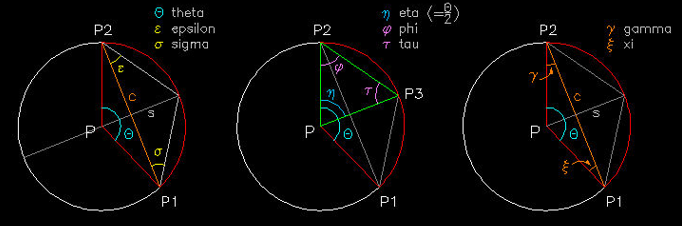
\includegraphics[width=1.0\textwidth]{figures/arcchord.png}
	\captionof{figure}{Дуга окружности с проведённой хордой и углами при ней}
	\label{fig:arcchord}
\end{figure}

Если провести к углу $\Theta$ биссектрису, то получится синий угол $\eta$. В итоге, мы получим равнобедренный треугольник (зеленый), в котором углы $\varphi$ и $\tau$ равны. Поскольку сумма углов в треугольнике всегда равна $180^{\circ}$ градусам, мы теперь знаем, что углы $\varphi$ и $\tau$ равны следующему (\ref{F:phi}):

\begin{equation}
	\varphi=\tau=\frac{(180^{\circ}-\frac{\Theta}{2})}{2}\Rightarrow\varphi=90^{\circ}-\frac{\Theta}{4}
	\label{F:phi}
\end{equation}

Теперь посмотрим на хорду $c$, проведённую от $P1$ до $P2$. Вместе с красными катетами угла $\Theta$ она тоже образует равнобедренный треугольник, а значит, $\gamma=\xi$. Угол при вершине треугольника $P-P1-P2$ --- это центральный угол $\Theta$, поэтому $\gamma$ и $\xi$ вычисляются следующим образом (\ref{F:gamma}):

\begin{equation}
	\gamma=\xi=\frac{180^{\circ}-\Theta}{2}\Rightarrow\gamma=90^{\circ}-\frac{\Theta}{2}
	\label{F:gamma}
\end{equation}

Таким образом, желтый угол $\varepsilon$ должен быть равняться разнице между фиолетовым углом $\varphi$ и оранжевым углом $\gamma$. Другими словами, $\varepsilon$ --- это четверть центрального угла $\Theta$ (\ref{F:epsilon}):

\begin{equation}
	\varepsilon=(90^{\circ}-\frac{\Theta}{4})-(90^{\circ}-\frac{\Theta}{2})\Rightarrow\varepsilon=\frac{\Theta}{2}-\frac{\Theta}{4}=\frac{\Theta}{4}
	\label{F:epsilon}
\end{equation}

Параметр \textit{bulge} (выпуклость) описывает, насколько дуга «выпирает» из вершин, то есть насколько велика высота дуги ($s$) (или расстояние от $P3$ до $P4$). Высота образует катет прямоугольного треугольника с углом, равным четверти центрального угла (см. желтый треугольник $P-P2-P3$ на рис. \ref{fig:epsilon}), и поскольку тангенс описывает отношение между катетами в прямоугольном треугольнике, легко описать геометрию с помощью этого одного угла (\ref{F:epsilon}):

\begin{equation}
	\frac{\sin(\varepsilon)}{\cos(\varepsilon)}=\tan(\varepsilon)
	\label{F:epsilon}
\end{equation}

\begin{figure}[H]
	\centering
	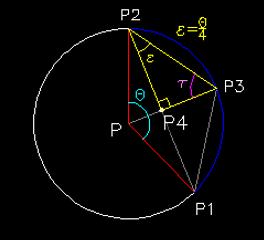
\includegraphics[width=0.5\textwidth]{figures/epsilon.png}
	\captionof{figure}{Связь угла $\varepsilon$ с центральным углом}
	\label{fig:epsilon}
\end{figure}

Мы, также, могли бы найти тангенс угла $\varepsilon$, просто разделив противолежащий катет на смежный катет --- что означает высоту дуги $s$, делённую на половину длины хорды $c$, --- но не зная $s$ и уже имея тангенс $\varepsilon$, полезнее найти $s$ (\ref{F:s}):

\begin{equation}
	s=\frac{c}{2}\cdot\tan(\varepsilon)
	\label{F:s}
\end{equation}

Примем

\begin{equation}
	\tan(\varepsilon)=bulge
	\label{F:tanepsilon}
\end{equation}

Тогда

\begin{equation}
	s=\frac{c}{2}\cdot bulge
	\label{F:sfinal}
\end{equation}

Таким образом, радиус дуги может быть найден следующим образом (\ref{F:r}):

\begin{equation}
	r=\frac{(\frac{c}{2})^2+s^2}{2s}
	\label{F:r}
\end{equation}

Знак той или иной выпуклости важен для определения дуги относительно вершин. Если выпуклость положительна, это означает, что дуга идёт против часовой стрелки от начальной вершины до конечной вершины. Если выпуклость отрицательна, это означает, что дуга идет, наоборот --- по часовой стрелке.

Поэтому все приведенные выше формулы должны касаться абсолютного значения выпуклости, а не фактического значения, иначе можно получить отрицательный радиус.

Итак, поняв, что $bulge = tan(\frac{\Theta}{4})$, в согласовании с документацией AutoCAD \cite{Autodesk} примем, что \textit{bulge} положителен, когда при передвижении от начальной точки дуги к конечной движение происходит против часовой стрелки.

Ясно, что когда $\Theta=0$, то и $bulge(\Theta)=0$. Для углов в $180^{\circ}$ условно принимается, что $bulge(\Theta)=\pm1$. В случае, когда $\Theta=90^{\circ}$, получим следующее (\ref{F:theta90}):

\begin{equation}
	bulge(90^{\circ})= \tan(\frac{90^{\circ}}{4})=\tan(\frac{\pi}{8})
	\label{F:theta90}
\end{equation}

Используя зависимость для тангенса половинного аргумента (\ref{F:tanhalfarg}):

\begin{equation}
	\tan(\frac{\alpha}{2})=\pm\frac{\sin(\frac{\alpha}{2})}{\cos(\frac{\alpha}{2})}=\pm\frac{2\sin^2(\frac{\alpha}{2})}{2\sin(\frac{\alpha}{2})\cos(\frac{\alpha}{2})}=\pm\frac{1-\cos(x)}{\sin(x)}
	\label{F:tanhalfarg}
\end{equation}

Для $\alpha=\frac{\pi}{8}$ получим (\ref{F:bulge90}):

\begin{equation}
	bulge(90^{\circ})=\tan(\frac{\pi}{8})=\pm\frac{1-\cos(\frac{\pi}{4})}{\sin(\frac{\pi}{4})}=\pm\frac{1-\frac{\sqrt2}{2}}{\frac{\sqrt2}{2}}=\pm\frac{1-\frac{1}{\sqrt2}}{\frac{1}{\sqrt2}}=\pm(\sqrt2-1)
	\label{F:bulge90}
\end{equation}



В результате, математические данные совпадают с документацией AutoCAD \cite{Autodesk} и гласят, что

\begin{enumerate}
	\item $bulge = 0$ для отрезка прямой,
	\item $bulge = \pm1$ для дуги в $180^{\circ}$ (половина окружности),
	\item $bulge = \pm(\sqrt2-1) \approx0.41421...$ для четвертей окружностей, когда угол раствора дуги равен $90^{\circ}$.
\end{enumerate}

%%% Local Variables:
%%% mode: latex
%%% TeX-master: "rpz"
%%% End:
